 \providecommand{\main}{../../..}
\documentclass[\main/main.tex]{subfiles}
\begin{document}
\subsection{Esercizio 1}
Dato il seguente problema di PL, si risolva graficamente e si ottenga il valore della soluzione ottima e di tutte le variabili di scarto.

Vi sono vertici ammissibili ai quali corrispondono basi degeneri?

Si ricavi, per via grafica, per quali valori di $b_3$, inizialmente pari a $-1$, la \textbf{composizione} della base ottima non cambia.

\begin{figure}
  \begin{align*}
    \max \quad -x_1 + x_2 \\
    -x_1 -x_2   & \leq -2 \\
    -x_1 + 3x_2 & \leq 6  \\
    -2x_1 + x_2 & \leq -1 \\
    4x_1 - x_2  & \leq 20 \\
    2x_1 + x_2  & \leq 16 \\
    x_1, x_2    & \geq 0
  \end{align*}
  \caption{Esercizio 1}
\end{figure}

\subsection{Soluzione esercizio 1}
\subsubsection*{Disegno l'area di definizione del problema}
\begin{figure}
  \begin{subfigure}{0.45\textwidth}
    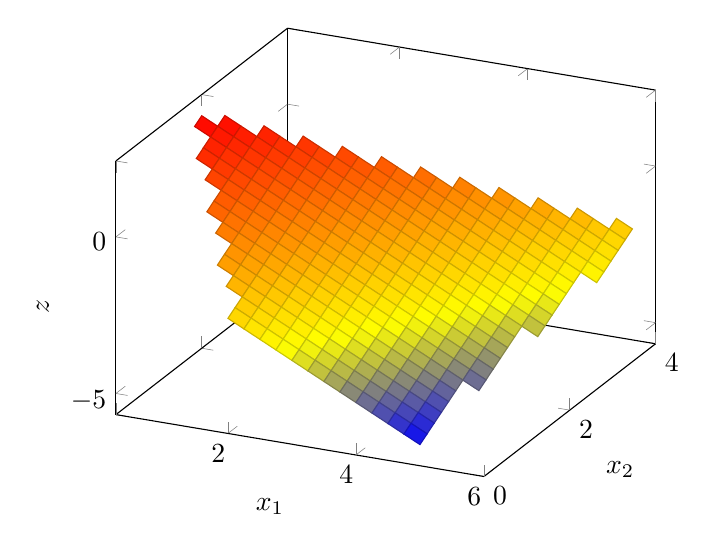
\begin{tikzpicture}
      \begin{axis}[
          xlabel=$x_1$,
          ylabel=$x_2$,
          zlabel=$z$,
          domain=0:6,
          y domain=0:4
        ]
        \addplot3[surf, unbounded coords=jump]
        {
          -x-y<=-2 &&
          -x +3*y <= 6 &&
          -2*x -y <= -1 &&
          4*x - y <= 20 &&
          2*x + y <= 16?
          -x+y:NaN
        };
      \end{axis}
    \end{tikzpicture}
    \caption{La funzione $z$}
  \end{subfigure}
  \begin{subfigure}{0.45\textwidth}
    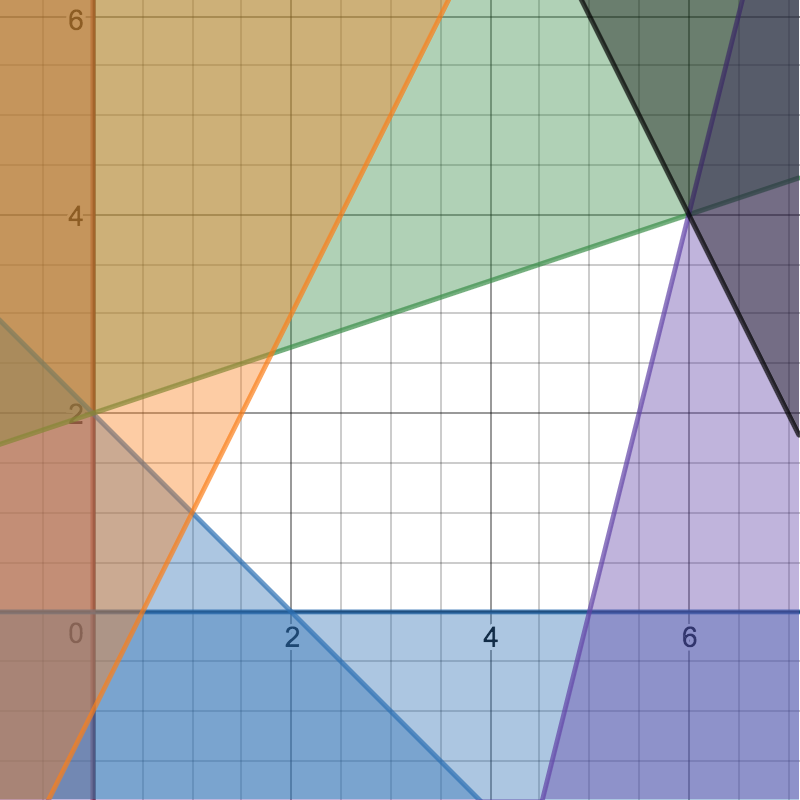
\includegraphics[width=0.8\textwidth]{2017_01_24}
    \caption{Regione di definizione del problema}
  \end{subfigure}
\end{figure}

\subsubsection*{Identifico la soluzione ottima}
Dall'area di definizione e dalla composizione della funzione si intuisce che il vincolo ottimo sarà quello con $x_1$ minimo e $x_2$ massimo. Procedo quindi a calcolare il valore assunto da $x_1$ e $x_2$ nell'intersezione tra il vincolo $2$ e $3$:

\[
  \begin{cases}
    -x_1 + 3x_2  = 6 \\
    -2x_1 + x_2  = -1
  \end{cases}
  \Rightarrow
  \begin{cases}
    -x_1 + 3(2x_1 -1)  = 6 \\
    x_2  =2x_1 -1
  \end{cases}
  \Rightarrow
  \begin{cases}
    5x_1 -3  = 9 \Rightarrow x_1 = \frac{9}{5} \\
    x_2  =2x_1 -1 \Rightarrow x_2 = \frac{18-5}{5} = \frac{13}{5}
  \end{cases}
\]

La soluzione ottima si trova nel vertice tra il vincolo $2$ e $3$ in $(\frac{9}{5}, \frac{13}{5})$ ed ha valore $z = \frac{13}{5} - \frac{9}{5} = \frac{4}{5}$.

\[
  z = \frac{4}{4}, \quad x_1 = \frac{9}{5}, \quad x_2 = \frac{13}{5}, \quad s_1 = \frac{12}{5}, \quad s_2 = 0, \quad s_3 = 0, \quad s_4 = \frac{49}{5}
\]

\subsubsection*{Identifico basi degeneri}
Una base è degenere quando in un vertice sono attivi più vincoli delle variabili esistenti. In questo caso, nel punto $(6,4)$ sono attivi 3 vertici.

\subsubsection*{Analisi di sensitività}
Modifica il valore di $b_3$ significa traslare il vincolo $3$, che è uno dei due che definisce il punto di ottimo $(\frac{9}{5}, \frac{13}{5})$. Non è pertanto possibile alterare il valore di $b_3$ senza modificare il valore ottimo.

Per quanto riguarda la composizione della base ottima, essa rimane invariata tra $b_{3_{max}}$ dove il vincolo $v_3$ incontra il vincolo $v_1$ nel punto $(0,2)$ e $b_{3_{min}}$ dove il vincolo $v_3$ incrocia $v_4$ nel punto $(6,4)$. Per calcolare il valore assunto da $b_3$ nei due punti di interesse è sufficiente sostituire i punti nella disequazione del vincolo.

\[
  b_{3_{max}} = -2(0) + 1(2) = 2 \qquad b_{3_{min}} = -2(6) + 1(4) = -8
\]
\end{document}